\documentclass{llncs}
\usepackage{amssymb}
\usepackage{url}
\usepackage{graphicx}

\title{Using Disjunctions in Association Mining}
\author{Martin Ralbovsk\'{y}\inst{1} \and Tom\'{a}\v{s} Kucha\v{r}\inst{2}}
\institute{Department of Information and Knowledge Engineering,\\
University of Economics, Prague, W. Churchill Sq.~4, 130 67 Praha~3, Czech Republic\\
\email{martin.ralbovsky@gmail.com}
\and
Department of Software Engineering, Faculty of Mathematics and Physics\\
Charles University, Malostransk� n�m. 25, 118 01 Prague, Czech Republic
\email{tomas.kuchar@gmail.com}
}

\begin{document}
\maketitle

\begin{abstract}
The paper focuses on usage of disjunction of items in association rules mining.
We used the GUHA method instead of the traditional \emph{apriori} algorithm and 
enhanced the former implementations of the method with ability of disjunctions setting
between items. Experiments were conducted in our Ferda data mining environment on data from
the medical domain. We found strong and meaningful association rules that could not be 
obtained without the usage of disjunction. 
\end{abstract}

{\small {\bf Keywords:} Association Mining, Disjunction, GUHA Method, Ferda}

\section{Introduction}
\label{section:introduction}
Association rules mining is an important technique widely used in the
KDD community \cite{KDNuggets}. Most of the tools nowadays use the \emph{apriori}
algorithm, or its modifications \cite{Agrawal1} \cite{Agrawal2}. The algorithm 
searches for frequent (or large) itemsets with given minimal \emph{support} and 
then calculates \emph{confidence}.
We will refer to this algorithm as to classical association mining. Its authors
considered only the conjunctions (and possibly negations) of items.

Yet sometimes it is feasible to examine disjunctions of items. Consider following
example: Medical expert wants to find associations between beer consumption and
other characteristics of a patient (blood pressure, level of cholesterol, body 
mass index...). The examined data contains information about consumption of 
three different types of beer: light 7 degree beer, drought 10 degree beer 
and lager 12 degree beer\footnote{This categorization of beer is traditional
in the Czech Republic and represents the weight percentage of mash in the end product.
7 degree beer contains about 2\% of alcohol, 10 degree beer about 3 to 4\% and 12
degree beer about 4 to 5\% of alcohol.}.
It is likely to happen that the number of patients
drinking 7 degree \emph{or} 12 degree beer is higher then the number of patients
drinking 7 degree \emph{and} 12 degree beer. 
More formally, from the rule $A \rightarrow B$ one can get rule $A \rightarrow B \vee C$
easily than the rule $A \rightarrow B \wedge C$. 
For semantically close entities\footnote{Drinking of different types of beer is
semantically close characteristics of a patient.} 
one can therefore use disjunctions and mine for rules 
with higher support (and possibly other characteristics).

The aim of this paper is to present an enhancement of classical association 
mining with the possibility of disjunction setting between the items. 
One cannot use \emph{apriori} for disjunctions, because the algorithm 
searches for frequent itemsets by binding items to already known itemsets
(of length \emph{k}) with conjunction to form itemsets (of length \emph{k+1}). We used
the older GUHA method instead, which mines for modifications of association rules.
The generalization enables disjunctions between items and had several partial 
implementations before the personal computer era. We created a new implementation
in our Ferda tool and conducted experiments with medical data using more strict 
requirements for rules than \emph{support} and \emph{confidence}. Meaningful rules have
been found; these rules could not be found without disjunction usage and have
interesting characteristics that should be subject of further research.

The paper is structured as follows: Section \ref{section:principles} explains the
GUHA method and its relation to classical association mining. Section \ref{section:ferda}
states a brief history of tools implementing the GUHA method leading to our Ferda tool.
Section \ref{section:experiments} describes conducted experiments. Section 
\ref{section:further} draws fields of further research and finally section
\ref{section:conclusion} concludes the work.

\section{Principles of association mining with GUHA}
\label{section:principles}

\subsection{The GUHA method}
\label{section:guha}
GUHA method is one of the first methods of exploratory data analysis, developed in 
the mid-sixties in Prague. The method has firm theoretical foundations based on 
observational calculi and statistics \cite{GUHA1}, \cite{GUHA2}. For purpose of 
this paper let us explain only the basic principles of the method, as shown in 
Figure \ref{fig:GUHA}.

\begin{figure}[ht]
\centering
\mbox{\resizebox{60mm}{!}{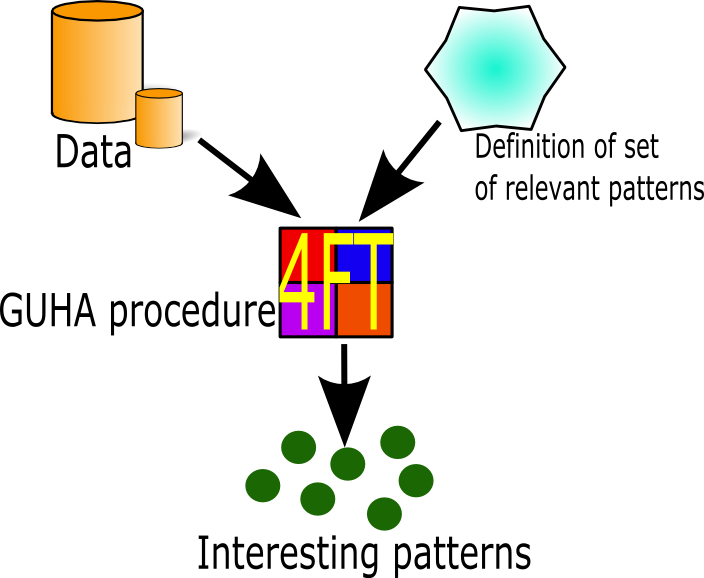
\includegraphics{GUHA.png}}}
\caption{The GUHA method}
\label{fig:GUHA}
\end{figure}

GUHA method is realized by GUHA procedures, located in the middle of the figure\footnote{
Even though we present only one GUHA procedure in this work, there are five more 
procedures working above one data table implemented in Ferda and also two relational
procedures under development.}. Inputs of the procedure are data and a simple definition
of a possibly large set of relevant patterns, which will be discussed in detail
in the following section \ref{section:patterns}. The procedure automatically generates
all the relevant patterns and verifies them against the provided data. Patterns that
are true are output of the procedure.

Although GUHA is not in principle restricted to mining association rules, the most 
used GUHA procedures mine for generalized  
association rules, as defined in \cite{Rauch}. Section \ref{section:4ft} introduces
4FT, procedure for association rules mining used in our work. Comparison study between
the classical association mining and mining using GUHA can be found in \cite{HajekHolena}.

\subsection{Definition of set of relevant patterns}
\label{section:patterns}
This section shows how set of relevant patterns is defined in association rules mining
with GUHA. We use the term attribute in the sense of \emph{categorial attribute}, i.e.
attribute with finite number of values.

\medskip
\textbf{Definition 1}
\emph{Let A be an attribute, A = $\{a_{1}, a_{2}...a_{n}\}$ and
$\alpha\subset A$, $\alpha\neq\emptyset$. Then $A(\alpha)$ is a}
\textbf{basic Boolean attribute}.

\textbf{Definition 2}
\emph{Each basic Boolean attribute is a }\textbf{Boolean 
attribute}\emph{. If $\alpha$ and $\beta$ are} \textsl{Boolean 
attributes}\emph{, $\alpha\wedge\beta$, $\alpha\vee\beta$ and
$\neg\alpha$ are }\textbf{Boolean attributes}.

\medskip
The above stated definition was introduced in \cite{Rauch} when
formalizing association rules. \emph{Boolean attributes} are used
as antecedents or succedents\footnote{In classical association mining 
called consequents.} in GUHA procedures, as will be described
in section \ref{section:4ft}. Our Ferda tool is the first program
to enable full \emph{Boolean attribute} definition including
disjunction and recursion. Example 1 shows us creation of 
\emph{Boolean attributes} from the beer consumption example from the
introduction.\\
\\
\textbf{Example 1}\\
The examined data includes three attributes: \textbf{beer7= $\{$no, low, high$\}$},\\
\textbf{beer10= $\{$no, low, high$\}$} and \textbf{beer12= $\{$no, low, high$\}$}
for consumption of 7, 10 and 12 degree beer respectively.\\
\\
Examples of \emph{basic Boolean attributes} are \textbf{beer7(no)},\\
\textbf{beer10(no, low)} or \textbf{beer12(high)}\footnote{Obviously, not all
the subsets of an attribute are meaningful to verify. Our method allows user to define
special subsets such as subsets with a given length, intervals, cyclic intervals or cuts
for ordinal data.}.\\
\\
Then we combine \emph{basic Boolean attributes} with logical operators to form
a rule:\\ 
\textbf{(beer7(no) $\vee$ beer10(no, low)) $\wedge$ $\neg$beer12(high)},\\ which is an example of \emph{Boolean attribute}.

\subsection{4FT procedure}
\label{section:4ft}
Classical association mining searches rules in form $X \longrightarrow Y$, where 
$X$ and $Y$ are sets of items. Procedure 4FT searches (in the simplified form) for 
rules in form \mbox{$\varphi \approx \psi$}, where $\varphi$ and $\psi$ are 
\emph{Boolean attributes} and $\approx$ is a \emph{4ft-quantifier}\footnote{The
more complex form includes another \emph{Boolean attribute} as a condition
In our work we do not mine for conditional rules, therefore we omit the more
complex definition.}. Relation \mbox{$\varphi \approx \psi$} is evaluated on the
basis of \emph{4ft table}, as shown in Table \ref{table:4FTcontingency}.

\begin{table}[ht]
	\begin{center}
		\begin{tabular}{r|c|c}
		{\b M}        & $ \psi $ &  $ \neg \psi $ \\
		\hline
		     $  \varphi $  &  \ \ $ a  \ \ $    & $  \ \ b \ \  $    \\
		\hline
		   $ \neg \varphi $  &  $ c $    & $ d $    \\
		\end {tabular}
	\end{center}
	
	\begin{center}
	Table 1: 4ft table
	\end{center}
	\caption{4FT contingency table}
	\label{table:4FTcontingency}
\end{table}

A \emph{4ft table} is a quadruple of natural numbers 
\emph{$\langle$a, b, c, d$\rangle$}
so that:

\begin{itemize}
	\item \emph{a}: number of objects (rows of \emph{M}) satisfying $\varphi$ and $\psi$
	\item \emph{b}: number of objects (rows of \emph{M}) satisfying $\varphi$ and not 
	satisfying $\psi$
	\item \emph{c}: number of objects (rows of \emph{M}) not satisfying $\varphi$ but 
	satisfying $\psi$
	\item \emph{d}: number of objects (rows of \emph{M}) satisfying neither $\varphi$ nor $\psi$
\end{itemize}

\emph{4ft-quantifier} expresses kind of dependency between $\varphi$ and $\psi$.
The quantifier is defined as a condition over the \emph{4ft table}.
By the expression \textbf{strict quantifier} we mean that there are no rules that
satisfy the quantifier in the usual case. Occurrence of such quantifier
means a very strong relation in the data.
In the following sections we present three quantifiers used in our work, the 
\emph{founded implication}, \emph{double founded implication} and 
\emph{founded equivalence} quantifiers\footnote{There are many other quantifiers
invented and implemented for the 4FT procedure.}. 
This part of the paper was 
greatly inspired by \cite{Kupka}, where detailed explanation of the most used
quantifiers can be found.

\subsection{Founded Implication Quantifier}
The founded implication is basic quantifier for the 4FT procedure introduced in
\cite{GUHA1} and is defined by following condition:

\begin{center}
	$\frac{a}{a+b+c+d}\geq Base \wedge \frac{a}{a+b} \geq p$
\end{center}

Here \emph{Base} and \emph{p} are threshold parameters of the procedure. As can
be seen, the \emph{Base} parameter corresponds to the \emph{support} and \emph{p} 
to the \emph{confidence} parameters 
of classical association mining. When using the 4FT procedure with \emph{founded
implication quantifier} and constructing \emph{Boolean attributes} only with
conjunctions, we get the same results as if using classical association mining.\\
\\
\textbf{Example 2}\\
Association rule \emph{Patients that drink 12 degree beer tend be overweight} 
is an example of rule we can found with \emph{founded implication}. This rule
can be formally written as \textbf{beer12(high) $\Rightarrow_{p,Base}$ BMI(overweight)}, 
where $\Rightarrow_{p,Base}$ stands for \emph{founded implication}.

\subsection{Double Founded Implication Quantifier}

The \emph{double founded implication} quantifier enriches the \emph{founded implication}
with symmetry feature. Symmetry means that when \mbox{$\varphi \approx \psi$} is
valid, when \mbox{$\psi \approx \varphi$} should be also valid. The quantifier has 
also threshold parameters $Base$ and $p$ and is defined by following condition:

\begin{center}
	$\frac{a}{a+b+c+d}\geq Base \wedge \frac{a}{a+b+c} \geq p$
\end{center}

We consider \emph{double founded implication} a \emph{strict quantifier}. 
However, we wanted to use the quantifier in our experiments to question the possibilities
of disjunctions.\\
\\
\textbf{Example 3}\\
The sign for \emph{double founded implication} quantifier is $\Leftrightarrow_{p,Base}$. The
rule \textbf{beer12(high) $\Leftrightarrow_{p,Base}$ BMI(overweight)} with the \emph{Boolean attributes} from example 2 can be verbally interpreted as \emph{Drinking 12
degree beer is in relation with being overweight among the patients}. 

\subsection{Founded Equivalence Quantifier}

The last presented quantifier is the \emph{founded equivalence}. It is
a stronger quantifier than \emph{founded implication} in terms of equivalence; ability
of two entities to attain the same logical values. The condition for the quantifier is

\begin{center}
	$\frac{a}{a+b+c+d}\geq Base \wedge \frac{a+d}{a+b+c+d} \geq p$
\end{center}

The fraction $\frac{a+d}{a+b+c+d}$ means the proportion of objects in the 
data matrix having $\varphi$ and $\psi$ both equal to 0 or 1, to all objects.
Similarly, $Base$ and $p$ are threshold parameters for the quantifier. As well
as \emph{double founded implication}, the \emph{founded equivalence} is 
considered to be a \emph{strict quantifier}.\\
\\
\textbf{Example 4}\\
The sign for the \emph{founded equivalence} quantifier is $\equiv_{p,Base}$. 
Generalized association rule \textbf{beer12(high) $\equiv_{p,Base}$
BMI(overweight)} can be translated to verbal form as \emph{Consumption
of 12 degree beer and being overweight has equivalent occurrence among
the patients}.

\section{GUHA and Ferda}
\label{section:ferda}
We would not achieve results presented in this work without 40 years long
research of the GUHA method and development of tools that implemented 
individual GUHA procedures. This section acknowledges achievements made
by researchers and developers in the past and briefly describes history that
lead to the state-of-the-art Ferda tool. See \cite{GUHAHistory} for more 
information about history of GUHA method.

The development of first GUHA procedure started in 1956. In modern terminology,
it mined for association rules with given \emph{confidence} with one item as a
succedent and one item as a consequent \cite{GUHAHistory}. The results, published
in \cite{GUHA1}, were clearly ahead of their time, long before terms like data
mining or knowledge discovery from databases were invented. 

First GUHA procedure to consider disjunctions was the IMPL procedure introduced
in \cite{GUHA2}. The procedure mined for rules in form \emph{CONJ} $\Rightarrow$
\emph{DISJ}, where \emph{CONJ} and \emph{DISJ} are elementary conjunctions and
disjunctions\footnote{Elementary conjunction is a conjunction made from one element
subsets of an attribute.}. $\Rightarrow$ is an \emph{implicational 
quantifier}\footnote{There are formal classes of \emph{4ft-quantifiers} defined in 
\cite{Rauch}. \emph{Implicational quantifiers} are one of the classes.}. The 
implementation of the procedure \cite{Ra:78} \cite{Granular} used for the 
first time the bit string approach\footnote{Also known as \emph{granular computing}.}. 
The input data were represented by strings of bits, which dramatically increased 
performance of the procedure.

The LISp-Miner tool\footnote{See \url{http://lispminer.vse.cz}.} started in 1996
and contributed greatly to the level of contemporary GUHA tools by implementing
six GUHA procedures and implementing coefficients. The latter technique allowed creation of
more general subsets of an attribute than one element subsets \cite{Alternative}
GUHA procedure 4ft-Miner implemented in LISp-Miner is predecessor of procedure 4FT 
introduced in this work. 4ft-Miner does not allow construction of 
\emph{Boolean attributes}, it constructs \emph{partial cedents} instead and until 
very recently it did not allow disjunctions. \emph{Partial cedent} is a restricted 
non recursive \emph{Boolean attribute}, more details are to be found in 
\cite{Alternative}. 

Ferda started as a student project to create a new visual environment for the
LISp-Miner system \cite{Ferda}. In the first version, creators used the LISp-Miner
GUHA procedures. The second version of the system, implemented in work \cite{Kuchar},
uses the bit string approach and enables full definition of \emph{Boolean attribute}.
It is the first modern tool (runs on personal computers) to implement disjunctions
and recursion of \emph{basic Boolean attributes}. The procedure 4FT implemented in
Ferda is the most generalized version of the original ASSOC procedure defined in 
\cite{GUHA2} The user environment is shown in Figure \ref{fig:Ferda}.

\begin{figure}[ht]
\centering
\mbox{\resizebox{100mm}{!}{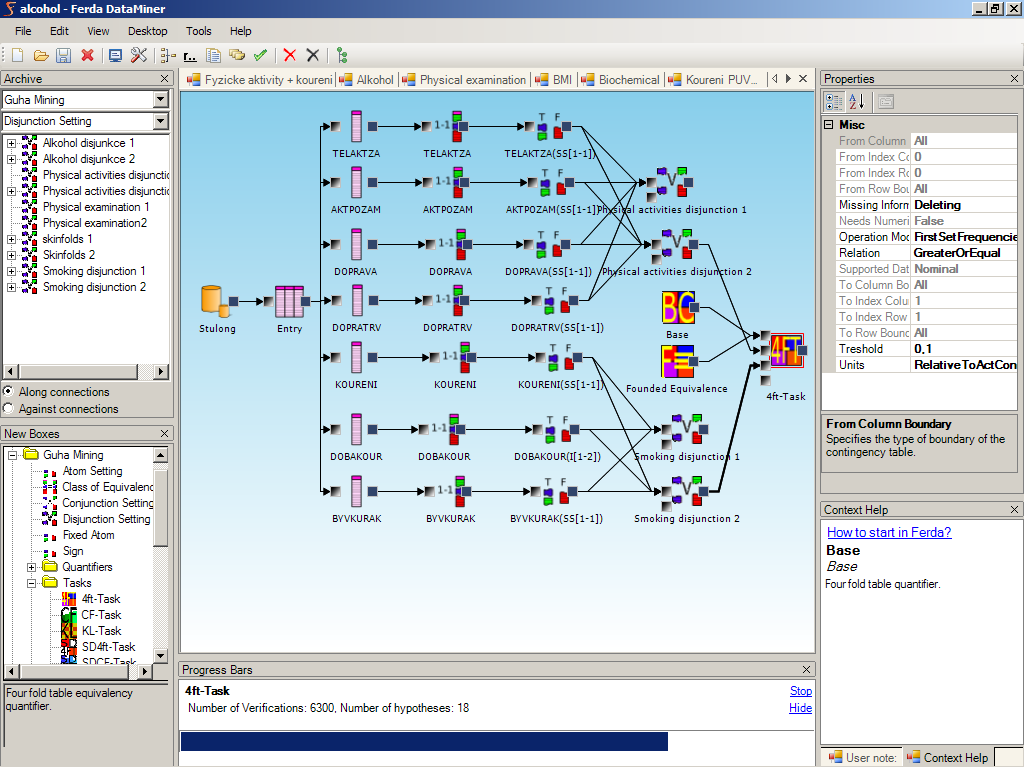
\includegraphics{Ferda.png}}}
\caption{Ferda environment}
\label{fig:Ferda}
\end{figure}

\section{Experiments}
\label{section:experiments}
In order to test the possibilities of disjunctions of items, we carried
out experiment, which consisted of testing number of analytical questions. 
We chose the STULONG data set, introduced in section \ref{section:STULONG}. 
The limitations and criteria that led to 
the experiment setup are described in sections \ref{section:limitations}
and \ref{section:setup}. Performance is discussed in section 
\ref{section:performance}. We found interesting and also some unexpected 
results which are summarized in section \ref{section:results}.

\subsection{STULONG Data Set}
\label{section:STULONG}

We decided to use the STULONG medical data set for our experiments\footnote{EUROMISE:
The STULONG Project \url{http://euromise.vse.cz/stulong}\\
The STULONG Project is partially supported by project no.LN00B107 of the Ministry of Education
of the Czech Republic and by grant no.2003/23 of the Internal Grant Agency of
the University of Economics, Prague. The STULONG study was carried out at the 2nd
Department of Medicine, 1st Faculty of Medicine of Charles University and Charles
University Hospital (head Prof. M. Aschermann, MD, SDr, FESC), under the supervision
of Prof. F. Boud\'{i}k, MD, ScD, with collaboration of M. Tome\v{c}kov\'{a}, MD, PhD
and Ass. Prof. J. Bultas, MD, PhD. The data were transferred to electronic form by
the European Centre of Medical Informatics, Statistics and Epidemiology of Charles
University and Academy of Sciences (head Prof. RNDr. J. Zv\'{a}rov\'{a}, DrSc).}.
The data set 
contains data about longitudinal study of atherosclerosis risk factors. 
There are two main reasons to choose this data set. First reason is that
STULONG is relativelly known among KDD researchers -- it served as the examined
data set for three ECML/PKDD discovery challenges. There are meaningful 
analytical questions defined on the data set to be examined, which is the
second reason. In our experiments we wanted to answer these questions. 

\subsection{Limitations}
\label{section:limitations}
Before explaining setup of the experiments, let us note two major limitations
of mining disjunctions in general. These limitations affect our experiments as
well. First limitation is generation of \emph{non prime} rules, in sense of GUHA mining 
\cite{GUHA2}.

\medskip
\textbf{Definition 3}
\emph{Let \mbox{$\varphi \approx \psi$} be a valid 4FT association rule and
$\varphi'$ and $\psi'$ are chosen normal forms of $\varphi$ and $\psi$.
The rule is} \textbf{prime} \emph{if the no $\varphi''\subset\varphi'$ and
$\psi''\subset\psi'$ exist, so that $\varphi'' \approx \psi''$ is a valid
4FT association rule.}

\medskip
Our implementation does not guarantee generation of prime rules. Therefore
we expect the number of valid rules to rise dramatically when using 
disjunctions with quantifiers that are not \emph{strict}. However, we may use
disjunctions with \emph{strict quantifiers}, where it is a common case that
no rules are found at all.

The other limitation is interpretation of rules with disjunction. The motivation
example of beer consumption in section \ref{section:introduction} showed that
it makes sense to use disjunctions with semantically close attributes, possibly
synonyms or taxonomically bound attributes. Interpretation of disjunction of
random attributes is rather problematic. Therefore we used for disjunctions
only the attributes of the same attribute groups\footnote{Groups of attributes, 
i.e. \emph{physical examination} are defined in the STULONG data set.}.

\subsection{Setup}
\label{section:setup}
From above stated limitations we concluded a setup for experiments. We answered
15 analytical questions concerning relations between significant characteristics
of patients' entry examination\footnote{The analytical questions
can be found at \url{http://euromise.vse.cz/challenge2004/tasks.html}}:

\medskip
\begin{enumerate}
	\item \emph{What are the relations between social factors and the following characteristics
	of men in the respective groups:}
	\begin{enumerate}
		\item \emph{Physical activity at work and in free time}
		\item \emph{Smoking}
		\item \emph{Alcohol consumption}
		\item \emph{BMI}
		\item \emph{Blood pressure}
		\item \emph{Level of total cholesterol, HDL cholesterol, triglycerides}
	\end{enumerate}
	\item \emph{What are the relations between physical activity at work and in free time
	and the following characteristics of men in the respective groups:}
	\begin{enumerate}
		\item \emph{Smoking}
		\item \emph{Alcohol consumption}
		\item \emph{BMI}
		\item \emph{Blood pressure}
		\item \emph{Level of total cholesterol, HDL cholesterol, triglycerides}
	\end{enumerate}
	\item \emph{What are the relations between alcohol consumption and the following
	characteristics of men in the respective groups:}
	\begin{enumerate}
		\item \emph{Smoking}
		\item \emph{BMI}
		\item \emph{Blood pressure}
		\item \emph{Level of total cholesterol, HDL cholesterol, triglycerides}
	\end{enumerate}
\end{enumerate}

The experiment consisted of two steps. The first tried to answer the questions
without usage of disjunctions. The second step used the task settings from 
the first step and allowed disjunctions of length 2. We applied the 
\emph{double founded implication} quantifier with settings \emph{p=0.9}, 
\emph{Base=0.1} and the \emph{founded equivalence} quantifier with 
settings \emph{p=0.9} and \emph{Base=0.1}. Below stated are the goals of
the experiment:

\begin{enumerate}
	\item Show the difference between using and not using disjunctions.
	\item Use disjunctions with \emph{strict quantifiers}.
	\item Find interesting rules that contain disjunction.
\end{enumerate}

\subsection{Performance}
\label{section:performance}
It is shown in \cite{Alternative} that the 4FT procedure operation time
without disjunctions is approximately linear to number of rows of the data
matrix. The reason is that pruning based on minimal support similar to one 
in \emph{apriori} algorithm is applied \cite{Alternative}. As was stated 
before, we cannot apply the same pruning with disjunctions, hence the operation time
rises with number of verifications. However, practical experience shows
that there is no need to be concerned, because the running times are
acceptable.

In our experiment we used a Pentium~M 1,7GHz processor with 1~GB of RAM
and Windows XP. We noted the running times of tasks designed to answer
proposed analytical questions. Without disjunctions, minimal running time
was 0.310 seconds, maximal running time was 2.543 seconds and average
running time was 0.829 seconds\footnote{Performance tests between 
the 4FT procedure implemented in Ferda and LISp-Miner can be found 
in \cite{Kuchar}.}. When using disjunctions, minimal running time was
0.370 seconds, maximal running time was 345,997 and average running time
was 38.9 seconds. In the maximum case, procedure constructed and verified
almost 8 million contingency tables. This is an abnormally big task setting; 
for majority of tasks, the number of verifications is between 5000 and 10000. 

\subsection{Results}
\label{section:results}
After conducting the first step of the experiment, we found 0 rules for 
14 of 15 analytical questions and one rule for question 3.(b). This result confirmed
our presumption, that \emph{double founded implication} and \emph{founded equivalence}
are \emph{strict quantifiers}. When using disjunctions, we found minimum 1 and maximum 
185 rules per analytical question. Although we agree that number of rules 
found is not a good metrics of measuring performance of new data mining technique, 
we think that the shift from zero rules found to non-zero rules found is significant. 

Let us consider the significance of the rules. In order
to reduce the amount of rules presented, we consider for simplicity only the
analytical question 3.(b). We may limit our analysis, because all the rules
found show similar characteristics. Possible rules answering the question
were presented as examples throughout the article. Moreover, a rule for this analytical
question was found during step one of the experiment.\\
\\
\emph{Beer7(No) $\Leftrightarrow_{p=0.986,Base=0.968}$ BMI(Normal weight, Overweight)}\\
\\
is the rule found without disjunction usage. It can be explained by the fact 
that 7 degree beer is very rare and it was mainly used for hydration of manual workers
in extremely hot working environment (glassmakers or metallurgists). Therefore majority
of population did not drink this type of beer. 

\begin{table}[ht]
	\centering
		\begin{tabular}{|p{4cm}|p{5cm}|p{0,8cm}|p{0,8cm}|p{0,8cm}|}
			\hline
			\textbf{Antecedent}&\textbf{Succedent}&\textbf{DFI}&\textbf{FE}&\textbf{Base}\\
			\hline
			Beer10(No) $\vee$ Beer12(No)&BMI(Normal weight, Overweight)&0.929&0.932&0.931\\
			\hline
			Beer12(No) $\vee$ Wine(Yes)&BMI(Normal weight, Overweight)&0.906&0.909&0.909\\
			\hline
			Beer12(No) $\vee$ Liquor(Yes)&BMI(Normal weight, Overweight)&0.905&0.908&0.909\\
			\hline
			Beer12(No) $\vee$&&&&\\
			Alcohol(Occasionally)&BMI(Normal weight, Overweight)&0.902&0.904&0.904\\
			\hline
			Beer12(No) $\vee$&&&&\\
			BeerDaily($<$1 liter)&BMI(Normal weight, Overweight)&0.946&0.948&0.948\\
			\hline
			Beer12(No) $\vee$&&&&\\
			WineDaily($<\frac{1}{2}$ liter)&BMI(Normal weight, Overweight)&0.9&0.903&0.903\\
			\hline
			Wine(No) $\vee$&&&&\\
			WineDaily($<\frac{1}{2}$ liter)&BMI(Normal weight, Overweight)&0.951&0.951&0.951\\
			\hline
			Liquor(No) $\vee$&&&&\\
			LiquorDaily($<$1 dL)&BMI(Normal weight, Overweight)&0.923&0.924&0.924\\
			\hline
		\end{tabular}
	\caption{Rules found}
	\label{tab:RulesFound}
\end{table}

Table \ref{tab:RulesFound} shows rules found with disjunction usage. The rules were
valid both for \emph{double founded implication} (DFI) and \emph{founded equivalence}(FE)
quantifiers. According to high values of both quantifiers and also to the high 
support of the rules (the \emph{Base} parameter), we have found very strong rules
containing disjunctions. Despite the initial concerns about interpretability of rules 
with disjunctions, the rules can be easily interpreted and comprehended. We are aware
of the fact, that the rules do not show any surprising relations\footnote{This may be
a problem of mining association rules in general.}. Yet they show strong relations
in data, where almost no relations without disjunction usage was discovered.

To conclude the experiment, all three goals from section \ref{section:setup} were
reached. We showed the difference of mining with and without disjunctions by 
getting almost none rules without disjunctions and more rules with disjunctions. We
managed to use \emph{strict quantifiers} and we also found interesting rules containing
disjunctions. The experiment also raised many questions about further development, some
of which will be discussed in the following section \ref{section:further}.

\section{Further research}
\label{section:further}
There are several directions to improve disjunctions using in association mining. 
This section explains the directions in more detail. The first direction
is optimalization of disjunctions verifications. We showed in section 
\ref{section:performance} that average running times for average size tasks
is acceptable. However there is still room for optimizing. As was stated before,
one cannot apply pruning used with conjunctions. Solution can lie in ordering 
of \emph{basic Boolean attributes} according to their support. However the
ordering itself can be a significant performance problem.

Another direction is to implement generation of prime rules only. 
The theory about prime rules is explained in \cite{GUHA2},
\cite{Rauch} includes information about deduction rules, which can be used when
checking prime property of an association rules. 

When evaluating results of our experiments, we came acros an interesting 
coincidence between values of quantifiers, mainly the \emph{Base} and \emph{p}
values of \emph{double founded implication} and \emph{founded equivalence}
quantifiers. A natural question occurs whether this is only a coincidence
or if it is some kind of functional dependence. The quantifiers are known
for years, yet without disjunctions we were not able on any data to mine 
a reasonable amount of rules to show the coincidence\footnote{This 
corresponds to considering the quantifiers as \emph{strict}.}.
Examination of quantifiers as functions $f:\Re^{4} \rightarrow \Re$ by 
finding functional extremes with the aid of calculus is another direction
of further research, which would answer the question of coincidence 
or dependence between quantifiers.

\emph{Boolean attribute} was presented in the article. The attribute
can reach values \emph{false} or \emph{true} (0 or 1). \emph{Fuzzy
attribute} can also be defined, reaching values from the interval
$<0,1>$. Then fuzzy \emph{4ft tables} can be constructed and fuzzy 
quantifiers can be defined\footnote{Naturally, some of the existing
quantifiers could not be used.}. \cite{Holena} is the inspiration
for this direction. 

Last, but not least direction of further research is cooperation 
with domain experts to evaluate usability of rules with disjunctions.
We mined over medical data and presented association rules comprehensible
to non medical experts. Presenting the rules found to the medical experts
provides valuable feedback for us. 

\section{Conclusion}
\label{section:conclusion}
We present an enhancement of association mining with the possibility
of setting disjunctions between the items. The classical \emph{apriori}
algorithm was not suitable for disjunctions. Instead older GUHA method
was applied. The 4FT procedure is used, which mines for rules in form
$\varphi \approx \psi$ where $\varphi$ and $\psi$ are \emph{Boolean
attributes} and $\approx$ is a \emph{4ft-quantifier}. \emph{Boolean
attribute} is a recursive structure, where disjunction can be used.
4FT procedure was implemented in our Ferda data mining tool. 

Experiments were conducted to show the usability of disjunctions
in association mining. We tried to answer number of analytical questions
from the STULONG medical data set containing statistical information
of atherosclerosis risk factors. We applied \emph{double founded
implication} and \emph{founded equivalence} quantifiers, which are
considered to be \emph{strict}, that is to return no rules in most cases. 
The experiments showed difference between mining with and without
disjunctions and found strong interpretable rules containing 
disjunctions in the data. The experiments also showed some issues, which
should be subjects of further research. 

\subsection*{Acknowledgements}
This work was supported by the project MSM6138439910 of the
Ministry of Education of the Czech Republic. We acknowledge the contribution
of our research colleagues Jan Rauch and Daniel Kupka for valuable comments and
reviews.

\begin{thebibliography}{20}

\bibitem{Agrawal1}
Agrawal R., Imielinski T., Swami A.:
\emph{Mining association rules between sets of items in large databases}.
Proc. of the ACM SIGMOD Conference on Management of Data, p.~207~--~216

\bibitem{Agrawal2}
Agrawal R., Mannila H., Srikant R., Toivonen H., Verkamo A.:
\emph{Fast discovery of association rules}. Fayyad, U., Piatetsky-Shapiro, G., Smyth, 
P., Uthurusamy, R., eds.: Advances in Knowledge Discovery and Data Mining. AAAI Press, 
Menlo Park (1996) p.~307~--~328

\bibitem{GUHAHistory}
H\'{a}jek P.: \emph{The GUHA Method in the Last Century and Now}. Znalosti 2006, 
Conference on Data Mining, Brno 2006, p.~10~--~20 (in Czech)

\bibitem{GUHA1}
H\'{a}jek P., Havel I., Chytil M.: \emph{The GUHA method of
automatic hypotheses determination}. Computing 1, 1966, p.~293~--~308

\bibitem{GUHA2}
H\'{a}jek P., Havr\'{a}nek, T.: \emph{Mechanising Hypothesis
Formation - Mathematical  Foundations  for  a   General  Theory}.
Springer-Verlag: Berlin  - Heidelberg - New York, 1978.

\bibitem{HajekHolena}
H\'{a}jek P., Hole\v{n}a M.: \emph{Formal logics of discovery and hypothesis 
formation by machine}. Theoretical Computer Science 292 (2003) p.~345~--~357

\bibitem{Holena}
Hole\v{n}a M.: \emph{Fuzzy hypotheses testing in framework of fuzzy logic}.
Fuzzy Sets and Systems, 149, p.~229~--~252

\bibitem{KDNuggets}
KDNuggets Polls, \emph{Data mining/analytic techniques you use frequently}.
\url{www.kdnuggets.com/polls/2005/data_mining_techniques.htm}

\bibitem{Ferda}
Kov\'{a}\v{c} M., Kucha\v{r} T., Kuzmin A., Ralbovsk\'{y} M.: \emph{Ferda, 
New Visual Environment for Data Mining}. Znalosti 2006, 
Conference on Data Mining, Hradec Kr\'{a}lov\'{e} 2006, p.~118~--~129 (in Czech)

\bibitem{Kuchar}
Kucha\v{r} T.: \emph{Experimental GUHA Procedures}, Master Thesis, 
Faculty of Mathematics and Physics, Charles University, Prague 2006 (in Czech)

\bibitem{Kupka}
Kupka D.: \emph{User support 4ft-Miner procedure for Data Mining}. Master Thesis,
Faculty of Mathematics and Physics, Charles University, Prague 2006 (in Czech)

\bibitem{Rauch}
Rauch J.: \emph{Logic of Association Rules}. In: Applied Inteligence, Vol. 22,
Issue 1, p.~9~--~28

\bibitem {Ra:78}
Rauch J.: \emph{Some Remarks on Computer  Realisations of GUHA Procedures}.
International Journal of Man-Machine Studies 10, 1978, p.~23~--~28

\bibitem{Alternative}
Rauch J., \v{S}im\accent23unek, M.: \emph{An Alternative Approach to Mining
Association Rules} Lin T Y, Ohsuga S, Liau C J, and Tsumoto S (eds):
Foundations of Data Mining and Knowledge Discovery, Springer-Verlag, 2005
p.~219~--~239

\bibitem{Granular}
Rauch J., \v{S}im\accent23unek, M.: \emph{GUHA Method and Granular Computing}.
Proceedings of IEEE International Conference on Granular Computing, 2005,
\url{http://www.cs.sjsu.edu/~grc/grc2005/index.html}

\end{thebibliography}

\end{document}